\documentclass[border=2mm]{standalone}
\usepackage{tikz}
\usepackage{pgfplots}
\pgfplotsset{compat=1.18}

\begin{document}

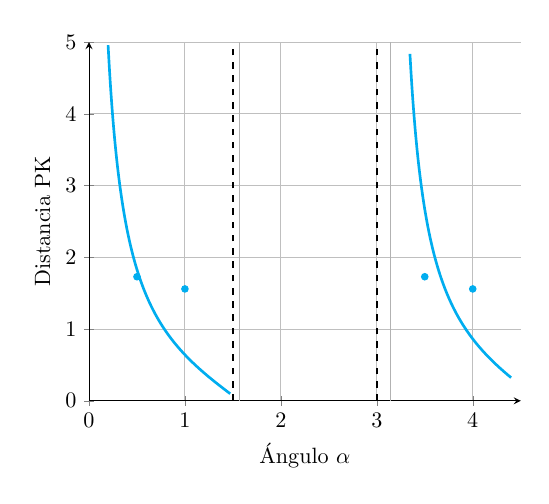
\begin{tikzpicture}[scale=0.8]
\begin{axis}[
    xlabel={Ángulo $\alpha$},
    ylabel={Distancia PK},
    xmin=0, xmax=4.5,
    ymin=0, ymax=5,
    grid=major,
    axis lines=left,
    samples=200,
    domain=0.1:4.4,
    restrict y to domain=0:5,
    unbounded coords=jump
]

% Función cotangente usando la técnica de R-bloggers con dominios separados
% Basado en el artículo "Some LaTeX Gems – Part 1: TikZ, Loops and more"

% Primera rama: desde 0.1 hasta antes de π/2 (≈1.57)
\addplot[cyan, very thick, smooth, domain=0.1:1.5, samples=100] {
    (deg(x) > 5 && deg(x) < 85) ? (1/tan(deg(x))) : nan
};

% Segunda rama: desde después de π/2 hasta antes de π (≈3.14)
\addplot[cyan, very thick, smooth, domain=1.65:3.1, samples=100] {
    (deg(x) > 95 && deg(x) < 175) ? (1/tan(deg(x))) : nan
};

% Tercera rama: desde después de π hasta antes de 3π/2 (≈4.71)
\addplot[cyan, very thick, smooth, domain=3.2:4.4, samples=100] {
    (deg(x) > 185 && deg(x) < 265) ? (1/tan(deg(x))) : nan
};

% Líneas punteadas verticales con etiquetas (como en la imagen original)
\draw[dashed, black, thick] (axis cs:1.5,0) -- (axis cs:1.5,5)
    node[above, black] {\small QP};
\draw[dashed, black, thick] (axis cs:3.0,0) -- (axis cs:3.0,5)
    node[above, black] {\small $I_1$};

% Asíntotas verticales en las discontinuidades (π/2, π, 3π/2)
\draw[gray!60, very thin] (axis cs:1.5708,0) -- (axis cs:1.5708,5);  % π/2
\draw[gray!60, very thin] (axis cs:3.1416,0) -- (axis cs:3.1416,5);  % π

% Puntos importantes en la curva (aproximados de la imagen original)
\addplot[cyan, mark=*, mark size=1.5pt, only marks] coordinates {
    (0.5,1.73) (1.0,1.56) (2.0,-1.73) (2.5,-0.36) (3.5,1.73) (4.0,1.56)
};

\end{axis}
\end{tikzpicture}

\end{document}
